\chapter{Plan de proyecto}

En este apartado se presenta la planificación seguida a lo largo de todo el proyecto. Se especifican una serie de tareas diferenciadas entre sí que a continuación serán detalladas en profundidad.\\ Para dar por finalizada una tarea, y así poder pasar a la siguiente, esta ha debido ser revisada previamente por el tutor. \\ Dentro del plan de estudios de la titulación, el trabajo de fin de grado tiene un peso de 12 créditos ECTS, y teniendo en cuenta que cada crédito ECTS equivale a 25 horas obtenemos que el proyecto debe ser completado en 300 horas. De esta manera la planificación que procederemos a desarrollar en esta sección, se elabora considerando que el horario va a ser de lunes a viernes con jornadas de 4 horas de trabajo.\\

\section{Descripcion de las tareas}
\subsection{Planificacion del proyecto}
\label{tareaPlanificacion}
La planificación del proyecto corresponde a la primera tarea. Se subdivide el proyecto en las propias tareas que se están comentando en este punto, se realiza una estimación de tiempo y se genera un diagrama de Gantt que se puede consultar en la figura \ref{fig:Gantt}.\\

Se estima que esta tarea tendrá una duración de 6 días.

\subsection{Estudio del algoritmo Box counting}
Con esta tarea se deja un tiempo para obtener formación sobre el algoritmo Box counting, conocer como funciona el \textit{"Fixed grid scan"}, y entender la implementación inicial escrita en Matlab. Para la realización de esta tarea se requiere de la adquisición de unas nociones básicas de Matlab debido al desconocimiento previo del lenguaje.\\

Se estima que esta tarea tendrá una duración de 4 días.

\subsection{Implementación en C++ del algoritmo Box counting}
Una vez se haya comprendido el funcionamiento del algoritmo con el que se va a trabajar a lo largo de todo el proyecto, se procederá a su implementación secuencial en C++. Dentro de esta tarea, entra la comprobación de la corrección del código implementado, comprobando que es válido y funciona correctamente con datos reales de activación cerebral.\\

Se estima que esta tarea tendrá una duración de 4 días.

\subsection{Experimentación y toma de tiempos del algoritmo sin paralelizar}
Se deja como tarea una etapa para la experimentación y toma de tiempos del algoritmo secuencial obtenido de la tarea anterior. Para la toma de tiempos se seguirá la metodología que se expone en el capítulo siguiente. El objetivo de la toma de tiempos del algoritmo secuencial es poder realizar comparaciones con las versiones que se implementen posteriormente, y medir que versión proporciona mejores aceleraciones.\\

Se estima que esta tarea tendrá una duración de 6 días.

\subsection{Paralelización del algoritmo con OpenACC}
Se planifica una tarea que conlleva la búsqueda de bibliografía y el estudio del estándar de programación OpenACC. El objetivo de esto es poder añadir al código secuencial las directivas OpenACC necesarias para explotar el paralelismo que nos aporta el uso de una CPU multicore.\\

Se estima que esta tarea tendrá una duración de 47 días.

\subsection{Experimentación y toma de tiempos de la paralelización con OpenACC}
Se planifica como tarea una etapa para la experimentación y toma de tiempos del código resultante de la tarea anterior. Además se analizarán los tiempos obtenidos y se compararán con los tiempos obtenidos en la etapa de experimentación del código secuencial mediante el cálculo de las aceleraciones.\\

Se estima que esta tarea tendrá una duración de 6 días.

\subsection{Paralelización del algoritmo con CUDA}
Se planifica una tarea que conlleva la búsqueda de bibliografía y el estudio de la plataforma de programación CUDA. De esta manera, en esta fase del proyecto, se implementará todo lo necesario para aprovechar la computación de propósito general en unidades de procesamiento gráfico (GPGPU) para aprovechar las tarjetas gráficas de la compañía Nvidia.\\

La paralelización con CUDA es un poco más compleja que la paralelización con OpenACC, por tanto, para realizar esta tarea se empezará implementado la versión en 2D, y partiendo de esa versión como base, se desarrollarán la versión 3D y 4D.\\

Se estima que esta tarea tendrá una duración de 47 días.

\subsection{Experimentación y toma de tiempos de la paralelización con CUDA}
Se deja como tarea una etapa para la experimentación y toma de tiempos del código resultante de la tarea anterior. Además se analizarán los tiempos obtenidos y se compararán con los tiempos obtenidos en la etapa de experimentación del código secuencial y con la etapa de experimentación del código paralelizado con OpenACC mediante el cálculo de las aceleraciones.\\

Se estima que esta tarea tendrá una duración de 6 días.

\subsection{Análisis de los resultados obtenidos}
El objetivo de esta tarea, es dejar un tiempo para la comparación de todos los resultados obtenidos en las etapas de experimentación y toma de tiempos, así como discusión y redacción de conclusiones sobre los resultados obtenidos.\\

Se estima que esta tarea tendrá una duración de 12 días.

\subsection{Elaboración de la memoria}
Durante el desarrollo de todo el proyecto se irá elaborando una memoria a modo de documentación del trabajo realizado.

\subsection{Preparación de la defensa ante el tribunal}
Tras la entrega del trabajo, se deja un tiempo para la elaboración del material necesario para la defensa y exposición del proyecto ante el tribubal.\\

Se estima que esta tarea tendrá una duración de 11 días.


\section{Diagrama de Gantt}
Como anticipábamos en \textit{"\nameref{tareaPlanificacion}"}, la primera etapa del proyecto es la planificación temporal del mismo. Para ello el primer paso es la división del proyecto en tareas y su correspondiente especificación.A continuación, se realiza una estimación de los días necesarios que tomará cada tarea, teniendo en cuenta que se trabajará en jornadas de 4 horas diarias de lunes a viernes. Finalmente, se hace una planificación temporal de todas las tareas en base a la estimación de tiempo realizada, obteniendo así el diagrama de la figura \ref{fig:Gantt}. En la tabla \ref{fig:presupuesto} se puede consultar la estimación de cada tarea así como, su fecha de inicio y finalización\\ Debido a la falta de experiencia en un proyecto de este tipo, esta especificación puede que no sea suficientemente detallada, en los siguientes capítulos se profundizará más en la descripción de las distintas tareas.\\

\begin{figure}[b]
    \centering
    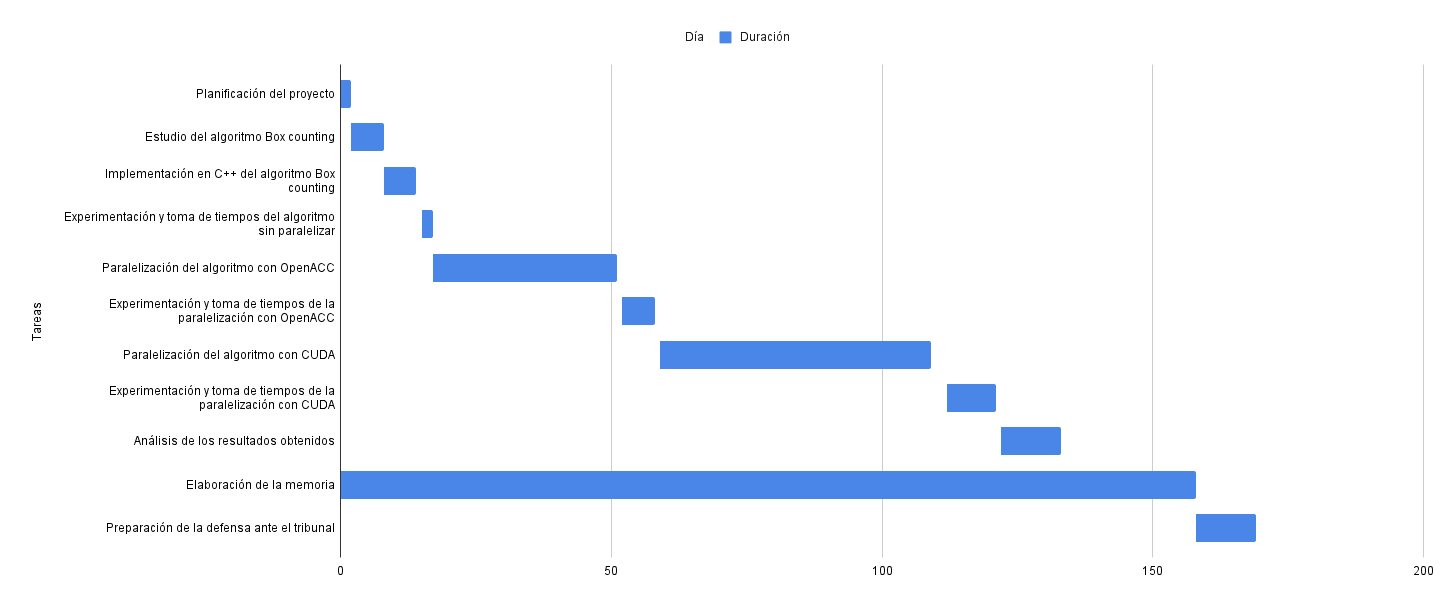
\includegraphics[width=\textwidth]{img/Diagrama de Gantt.png}
    \caption{Diagrama de Gantt}
    \label{fig:Gantt}
\end{figure}

\begin{table}[H]
    \centering
    \begin{adjustbox}{angle=90, max height=\textheight}
    \begin{tabular}{|clllrrl|} 
    \hline
    \rowcolor{black} \multicolumn{1}{|l}{}  & \textcolor{white}{Tareas} & \textcolor{white}{Fecha de inicio}         & \textcolor{white}{Fecha de finalización} & \textcolor{white}{Duración en días}&\\                                      
    \hline
    \rowcolor{white} \multicolumn{1}{|l}{}  & \textcolor{black}{Planificación del proyecto} & \textcolor{black}{1/2/2021}         & \textcolor{black}{7/2/2021} & \textcolor{black}{6}&\\
    \hline
    \rowcolor{white} \multicolumn{1}{|l}{}  & \textcolor{black}{Estudio del algoritmo Box counting} & \textcolor{black}{1/2/2021}         & \textcolor{black}{5/2/2021} & \textcolor{black}{4}&\\  
    \hline
    \rowcolor{white} \multicolumn{1}{|l}{}  & \textcolor{black}{Implementación en C++ del algoritmo Box counting} & \textcolor{black}{2/2/2021}         & \textcolor{black}{11/2/2021} & \textcolor{black}{9}\\
    \hline
    \rowcolor{white} \multicolumn{1}{|l}{}  & \textcolor{black}{Experimentación y toma de tiempos del algoritmo sin paralelizar} & \textcolor{black}{11/2/2021}         & \textcolor{black}{17/2/2021} &\textcolor{black}{6}&\\
    \hline
    \rowcolor{white} \multicolumn{1}{|l}{}  & \textcolor{black}{Paralelización del algoritmo con OpenACC} & \textcolor{black}{18/2/2021}         & \textcolor{black}{6/4/2021} &\textcolor{black}{47}\\
    \hline
    \rowcolor{white} \multicolumn{1}{|l}{}  & \textcolor{black}{Experimentación y toma de tiempos de la paralelización con OpenACC} & \textcolor{black}{6/4/2021}         & \textcolor{black}{13/4/2021} &\textcolor{black}{6}\\
    \hline
    \rowcolor{white} \multicolumn{1}{|l}{}  & \textcolor{black}{Paralelización del algoritmo con CUDA} & \textcolor{black}{13/4/2021}         & \textcolor{black}{30/5/2021} &\textcolor{black}{47}\\
    \hline
    \rowcolor{white} \multicolumn{1}{|l}{}  & \textcolor{black}{Experimentación y toma de tiempos de la paralelización con CUDA} & \textcolor{black}{31/5/2021}         & \textcolor{black}{7/6/2021} &\textcolor{black}{6}\\
    \hline
    \rowcolor{white} \multicolumn{1}{|l}{}  & \textcolor{black}{Análisis de los resultados obtenidos} & \textcolor{black}{8/6/2021}         & \textcolor{black}{20/6/2021} &\textcolor{black}{12}&\\
    \hline
    \rowcolor{white} \multicolumn{1}{|l}{}  & \textcolor{black}{Elaboración de la memoria} & \textcolor{black}{1/2/2021}         & \textcolor{black}{9/7/2021} &\textcolor{black}{-}&\\
    \hline
    \rowcolor{white} \multicolumn{1}{|l}{}  & \textcolor{black}{Preparación de la defensa ante el tribubal} & \textcolor{black}{9/7/2021}         & \textcolor{black}{20/7/2021} &\textcolor{black}{11}&\\                                  
    \hline
    \end{tabular}
    \end{adjustbox}
    \caption{Planificación temporal de las tareas}
    \label{fig:presupuesto}
\end{table}

\section{Recursos}
\subsection{Recursos Humanos}
Para la realización del proyecto se cuenta con Miguel Ángel Posadas Arráez como autor del mismo, y con el Profesor Dr. Juan Ruiz de Miras como tutor encargado de la supervisión del mismo.

\subsection{Recursos Software}
Debido a que este proyecto corresponde al ámbito académico, se presta especial atención en utilizar herramientas con licencia libre, o que sean accesibles mediante la adquisición de algún tipo de licencia de estudiante, beneficiandonos así, de las ventajas que nos proporciona pertenecer a la Universidad de Granada.\\

\begin{itemize}
    \item Como alternativa a Matlab, se utiliza Octave. \cite{unknown-author-2021B}.
    \item Como herramienta de control de versiones, se utiliza GitHub, siendo posible obtener una licencia de estudiante en la siguiente referencia \cite{unknown-author-2021}.
    \item Para la gestión del proyecto y la gestión de toda la documentación, se utiliza la suite ofimática de Google, accediendo siempre con la cuenta corporativa de la Universidad de Granada (dominio go.ugr.es).
    \item Para la paralelización mediante el uso de tarjeta gráfica, se utiliza el CUDA Toolkit, \cite{unknown-author-no-date}.
    \item Para la paralelización mediante el uso de los mútliples núcleos de la CPU, se utiliza OpenACC. \cite{unknown-author-no-dateB}.
\end{itemize}

\subsection{Recursos Hardware}
Para el desarrollo del proyecto se utiliza un ordenador portátil, que cuenta con las siguientes características:

\begin{itemize}
    \item Sistema Operativo: Ubuntu 20.04.2 LTS
    \item CPU: Intel(R) Core(TM) i7-7700HQ CPU @ 2.80GHz
    \item GPU: Nvidia GeForce GTX 1050 Mobile
    \item Memoria RAM: 12 GB DDR4
    \item Almacenamiento secundario:
    \begin{itemize}
        \item SSD NVMe LITEON CA1-8D128-HP 128GB
        \item SSD Samsung SSD 860 QVO 1TB
    \end{itemize} 
\end{itemize}

Con el objetivo de dejar más información sobre la plataforma en la que se desarrolla el proyecto, se deja la figura \ref{fig:CPU} con la salida de la ejecución del comando lscpu, y la figura \ref{fig:GPU} con la salida del comando pgaccelinfo.

\begin{figure}[H]
    \centering
    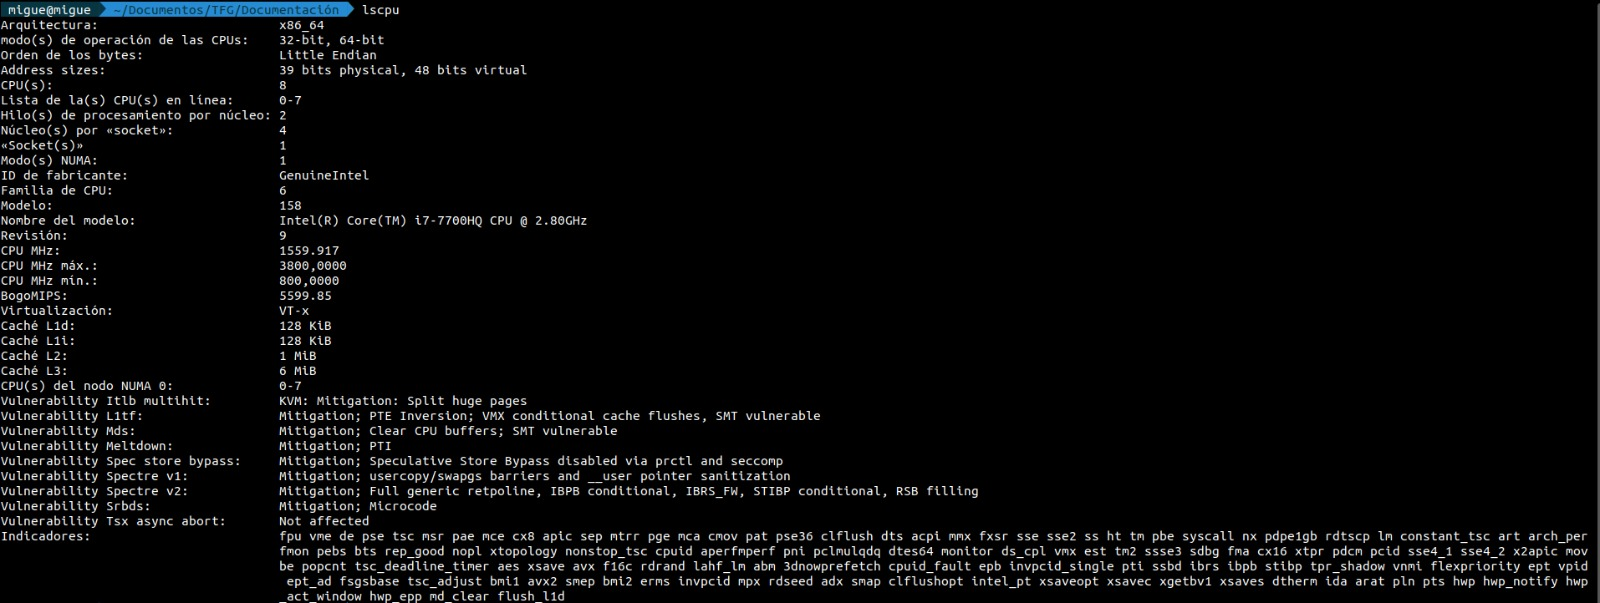
\includegraphics[width=\textwidth]{img/lscpu.jpeg}
    \caption{Salida comando lscpu}
    \label{fig:CPU}
\end{figure}

\begin{figure}[H]
    \centering
    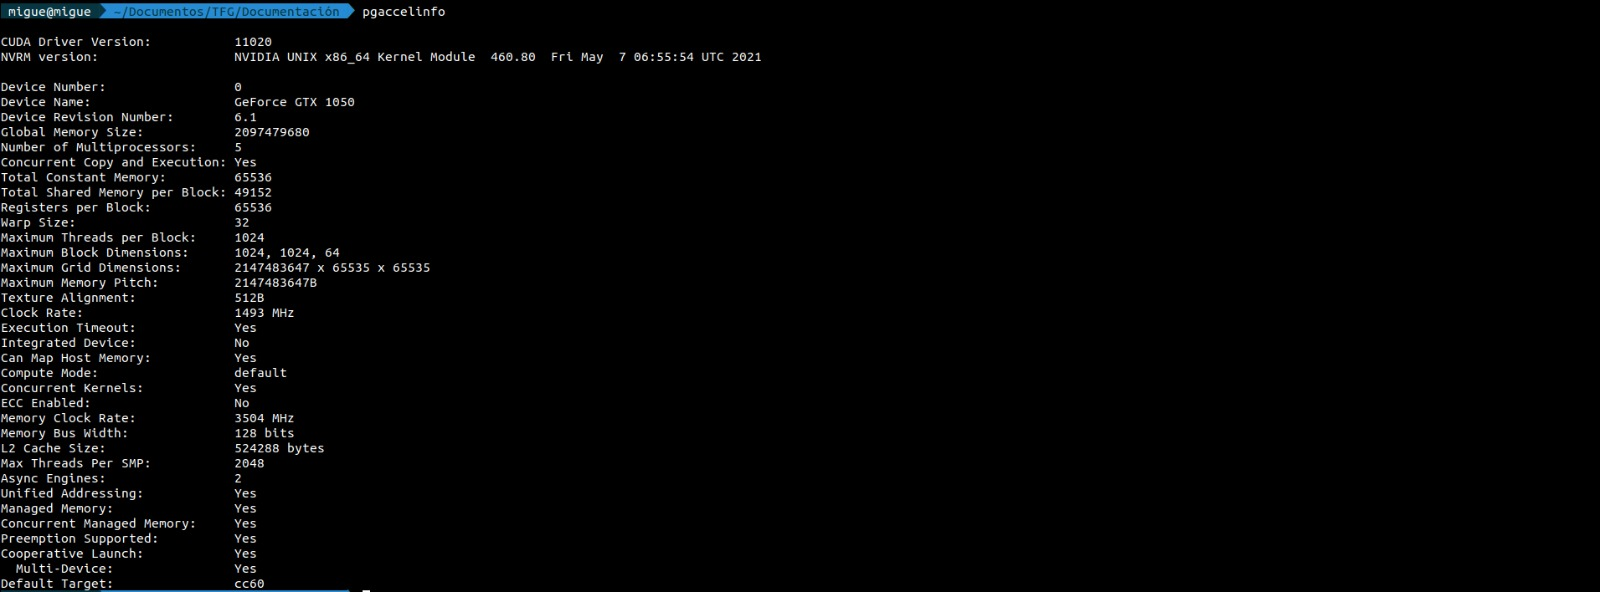
\includegraphics[width=\textwidth]{img/pgaccelinfo.jpeg}
    \caption{Salida comando pgaccelinfo}
    \label{fig:GPU}
\end{figure}

